% arara: pdflatex
% arara: convert: {density: 160, otheroptions: -dispose previous -delay 25 -loop 1, format: gif}
% xarara: showfile: {format: gif}
\documentclass{beamer}
\setbeamertemplate{navigation symbols}{}
\usepackage{tikzducks}
\usetikzlibrary{arrows.meta}
\usetikzlibrary{positioning,shapes.callouts}

\newcommand{\devilduck}{%
\begin{scope}
\clip (0,0) -- ++(2.2,0) -- ++(0,2.6) -- ++(-2.2,0) -- cycle;
\duck[body=red, grumpy, bill=black, name=devil]
\filldraw[black] ([xshift=2pt]devil-head) to[bend right] +(6pt,6pt) to[bend left] +(-4pt,-8pt) to[bend left] cycle;
\filldraw[black] ([xshift=-2pt, yshift=1pt]devil-head) to[bend left] +(-6pt,6pt) to[bend right] +(4pt,-8pt) to[bend right] cycle;
\end{scope}%
}
\newcommand{\normalduck}{%
\begin{scope}[xshift=-11em]
\clip (0,0) -- ++(2.2,0) -- ++(0,2.6) -- ++(-2.2,0) -- cycle;
\duck[name=duck]	
\end{scope}%
}
\newcommand{\fork}[1]{%
\coordinate (forkpos) at ([xshift={#1}]devil-wing);
\draw[-Stealth, line width=1.6pt] (forkpos) -- ++(-2.5,0);
\draw[Stealth-Stealth, line width=1.6pt] ([shift={(-2.3,.3)}]forkpos) -- ++(.6,0) to[bend left]  ++(0,-.6) -- ++(-.6,0);%
}

\begin{document}
\begin{frame}
	\frametitle{Devil Ducks}
	\centering
	
\begin{tikzpicture}	
	\devilduck
	\normalduck
	\fork{1em}
	\end{tikzpicture}	
\end{frame}
\begin{frame}
\frametitle{Devil Ducks}
\centering
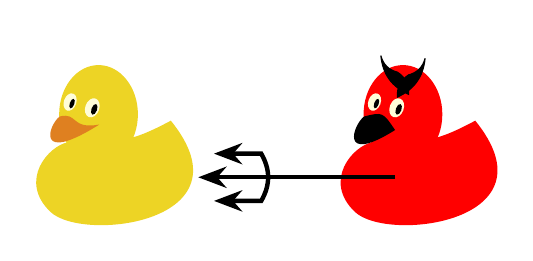
\begin{tikzpicture}
	\devilduck
	\normalduck
	\fork{0em}
\end{tikzpicture}
\end{frame}
\begin{frame}
\frametitle{Devil Ducks}
\centering

\begin{tikzpicture}[remember picture]
\devilduck
\normalduck
\fork{-1em}
\end{tikzpicture}
\begin{tikzpicture}[remember picture, overlay]
\node[ellipse callout, draw=blue, text=red] at ([shift={(-1,1)}]duck-head) {Ouch!};
\end{tikzpicture}
\end{frame}
\end{document}
